\documentclass{ExcelAtFIT}
%\documentclass[czech]{ExcelAtFIT} % when writing in CZECH
%\documentclass[slovak]{ExcelAtFIT} % when writing in SLOVAK


%--------------------------------------------------------
%--------------------------------------------------------
%	REVIEW vs. FINAL VERSION
%--------------------------------------------------------

%   LEAVE this line commented out for the REVIEW VERSIONS
%   UNCOMMENT this line to get the FINAL VERSION
%\ExcelFinalCopy


%--------------------------------------------------------
%--------------------------------------------------------
%	PDF CUSTOMIZATION
%--------------------------------------------------------

\hypersetup{
	pdftitle={Paper Title},
	pdfauthor={Author},
	pdfkeywords={Keyword1, Keyword2, Keyword3}
}

\lstset{
	backgroundcolor=\color{white},   % choose the background color; you must add \usepackage{color} or \usepackage{xcolor}; should come as last argument
	basicstyle=\footnotesize\tt,        % the size of the fonts that are used for the code
}

\definecolor{codegray}{rgb}{0.5,0.5,0.5}
\definecolor{codepurple}{rgb}{0.58,0,0.82}
\definecolor{backcolour}{rgb}{0.95,0.95,0.92}
\lstdefinestyle{pythonStyle}{
    backgroundcolor=\color{backcolour},
    commentstyle=\color{codegreen},
    keywordstyle=\color{blue},
    numberstyle=\tiny\color{codegray},
    stringstyle=\color{codepurple},
    basicstyle=\ttfamily\footnotesize,
    breakatwhitespace=false,
    breaklines=true,
    captionpos=b,
    keepspaces=true,
    numbers=right,
    showspaces=false,
    showstringspaces=false,
    showtabs=false,
    tabsize=2
}


%--------------------------------------------------------
%--------------------------------------------------------
%	ARTICLE INFORMATION
%--------------------------------------------------------

\ExcelYear{2022}

\PaperTitle{ENOSS - Event Notifications in OpenStack Swift}

\Authors{Nemanja Vasiljević*}
\affiliation{*%
  \href{mailto:xvasil03@stud.fit.vutbr.cz}{xvasil03@stud.fit.vutbr.cz},
  \textit{Faculty of Information Technology, Brno University of Technology}}
%%%%--------------------------------------------------------
%%%% in case there are multiple authors, use the following fragment instead
%%%%--------------------------------------------------------
%\Authors{Jindřich Novák*, Janča Dvořáková**}
%\affiliation{*%
%  \href{mailto:xnovak00@stud.fit.vutbr.cz}{xnovak00@stud.fit.vutbr.cz},
%  \textit{Faculty of Information Technology, Brno University of Technology}}
%\affiliation{**%
%  \href{mailto:xdvora00@stud.fit.vutbr.cz}{xdvora00@stud.fit.vutbr.cz},
%  \textit{Faculty of Information Technology, Brno University of Technology}}

\Keywords{Event --- Notifications --- OpenStack Swift}

\Supplementary{\href{http://youtu.be/S3msCdn3fNM}{Demonstration Video} --- \href{http://excel.fit.vutbr.cz/}{Downloadable Code}}


%--------------------------------------------------------
%--------------------------------------------------------
%	ABSTRACT and TEASER
%--------------------------------------------------------

\Abstract{

%What is the problem? What is the topic?, the aim of this paper?
%Currently there is no way for users to have any informations about events occuring in parts of object storage that they own/have access to in OpenStack Swift and OpenIO SDS. Swift and OpenIO SDS do not provide any informations to owners(or other allowed parties) when content of their object storage is accessed, changed, created or deleted.

Currently object storage OpenStack Swift does not provide any informations to users about events occured in storage they own/have access to. Users do not have information when content of their object storage is accessed, changed, created or deleted.
The aim of this paper is to create solution that will send notifications about events occured in OpenStack Swift to user specified destinations.
%How is the problem solved, the aim achieved (methodology)?
Proposed solution, using metadata, allows users to specify where and which event should be pubslished based on even types (read, create, modify, delete) and other properties such as object prefix, suffix, size, etc. It also offers mutiple destinations(Beanstalkd queue, Kafka, etc.) to which notifications can be publsihed.
%What are the specific results? How well is the problem solved?
Solution is fully compatible with AWS S3 Event Notifications and compared to AWS supports more destinations, event types, filters and allows unsuccessful events to be published as well.
%So what? How useful is this to Science and to the reader?
Event notification can be used not just for monitoring, but also for automatization and serverless computing similarly to AWS Lambda.
}


\Teaser{
	\TeaserImage{placeholder.pdf}
	\TeaserImage{placeholder.pdf}
	\TeaserImage{placeholder.pdf}
}



%--------------------------------------------------------
%--------------------------------------------------------
%--------------------------------------------------------
%--------------------------------------------------------
\begin{document}

\startdocument


%--------------------------------------------------------
%--------------------------------------------------------
%	ARTICLE CONTENTS
%--------------------------------------------------------

%--------------------------------------------------------
%--------------------------------------------------------
%--------------------------------------------------------
%--------------------------------------------------------
\section{Introduction} \label{introduction}

% Questions to answer:
% - why now? skip?
% - why this? skip??
% - why this way?
% - why should reader care?
% Important: Story telling!


%\textbf{[Motivation]} What is the raison d'\^{e}tre of your project? Why should anyone care? No general meaningless claims. Make bulletproof arguments for the importance of your work.

Object storage is data storage architecture that manages data as objects, and each object typically includes data itself and some additional information stored in objects metadata. Since object storages are often used in cloud computing, data are stored in remote locations, to which users do not have direct and complete access, some users or external services might want to receive information about specific events in storages where their data are located. For example, currently there is no easy way to detect changes in specific container, except to list it's content and compare timestamps, which can be complex, slow and unefficient if there is a lot objects in storage.

The importance of this work is to provide event information to users in OpenStack Swift, which will allow users to react to those events, create more sophisticated backend operations, postprocessing and automatization, or possibly prevent/detect unwanted actions. In addition, providing event notifications will allow users to have a better picture of what is going on in their storage and improve monitoring in object storage.

%\textbf{[Problem definition]} What exactly are you solving? What is the core and what is a bonus? What parameters should a proper solution of the problem have? Define the problem precisely and state how its solution should be evaluated.

Users can be interested in only specific events, for example creating of new objects in container, therefore it is important that proposed solution allows event filtering based on event type and other properties (e.g. object name prefix/suffix/size). Since object storage have multiple users, each user can have different requirements for event notification and proposed solution must be prepared for it.

Application of event notifications is various, from simple monotoring or webhook, to more sophisticated application as serverless computing like AWS Lambda. This means that structure of event notification may differ based on its application and destination to which is published. Proposed solution must be ready to pubslih event notification to different destinations as well as in different event notfication structure.

AWS S3 object storage is one of the most popular storage with their own API, that is supported by many other object storages including OpenStack Swift. Since AWS S3 supports event notifications, it would be ideal if proposed solution in OpenStack is compatible with S3 event notification protocol. This would allow easier transfer users from AWS S3 to OpenStack Swift. As result, not only that OpenStack Swift would offer same functionality as AWS S3 (that currently lacks), but protocol would be compatible with AWS S3, which would allow easier tranfer users from AWS S3 to OpenStack Swift. Therefore users would not have to learn additional protocol, and can follow existing AWS S3 which is most popular and well documented.


\section{OpenStack Swift}

OpenStack Swift is open-source object storage developed by Rackspace, a company that, together with NASA, created the OpenStack project. After becoming an open-source project, Swift became the leading open-source object storage supported and developed by many famous IT companies, such as Red Hat, HP, Intel, IBM, and others.

OpenStack Swift is a multi-tenant, scalable, and durable object storage capable of storing large amounts of unstructured data at low cost\cite{swiftOpenStackSwift}.

\subsection{Data model}

OpenStack Swift allows users to store unstructured data objects with a canonical name containing \textit{account}, \textit{container} and \textit{object} in given order\cite{swiftOpenStackSwift}. The account names must be unique in the cluster, the container name must be unique in the account space, and the object names must be unique in the container. Other than that, if containers have the same name but belong to a different account, then they represent different storage locations. The same principle applies to objects. If objects have the same name but not the same container and account name, then these objects are different.

\textbf{Accounts} are root storage locations for data. Each account contains a list of containers within the account and metadata stored as key-value pairs. Accounts are stored in the account database. In OpenStack Swift, account is \textbf{storage account} (more like storage location) and \textbf{do not represent a user identity}\cite{swiftOpenStackSwift}.

\textbf{Containers} are user-defined storage locations in the account namespace where objects are stored. Containers are one level below accounts, therefore they are not unique in the cluster. Each container has a list of objects within the container and metadata stored as key-value pairs. Containers are stored in container database\cite{swiftOpenStackSwift}.

\textbf{Objects} represent data stored in OpenStack Swift. Each object belongs to one (and only one) container. An object can have metadata stored as key-value pairs. Swift stores multiple copies of an object across the cluster to ensure durability and availability. Swift does this by assigning an object to \textit{partition}, which is mapped to multiple drives, and each driver will contain object copy\cite{swiftOpenStackSwift}.


\subsection{Main processes}
The path towards data in OpenStack Swift consists of four main software services: \textbf{Proxy server}, \textbf{Account server}, \textbf{Continaer server} and \textbf{Object server}. Typically Account, Container and Object server are located on same machine creating \textbf{Storage node}.

\textbf{Proxy server} is the service responsible for communication with external clients. For each request, it will look up storage location(node) for an account, container, or object and route the request accordingly\cite{SwiftArchitecturalOverview}. The proxy server is responsible for handling many failures. For example, when a client sends a \texttt{PUT} request to OpenStack Swift, the proxy server will determine which nodes store the object. If some node fails, a proxy server will choose a hand-off node to write data. When a majority of nodes respond successfully, then the server proxy will return a success response code\cite{swiftOpenStackSwift}.

\textbf{Account server} stores information about containers in a particular account to SQL database. It is responsible for listing containers. It does not know where specific containers are, just what containers are in an account\cite{SwiftArchitecturalOverview}.

\textbf{Container server} is similar to account server, except it is responsible for listing objects and also does not know where specific objects are\cite{SwiftArchitecturalOverview}.

\textbf{Object Server} is blob storage capable of storing, retrieving, and deleting objects. Objects are stored as binary files to a filesystem, where metadata are stored in the \textit{file's extended attributes (xattrs)}. This requires a filesystem with support of such attributes. Each object is stored using a hash value of object path (account/container/object) and timestamp. This allows storing multiple versions of an object. Since last write wins (due to timestamp), it is ensured that the correct object version is served\cite{SwiftArchitecturalOverview}.

\begin{figure}[t]
		\centering
		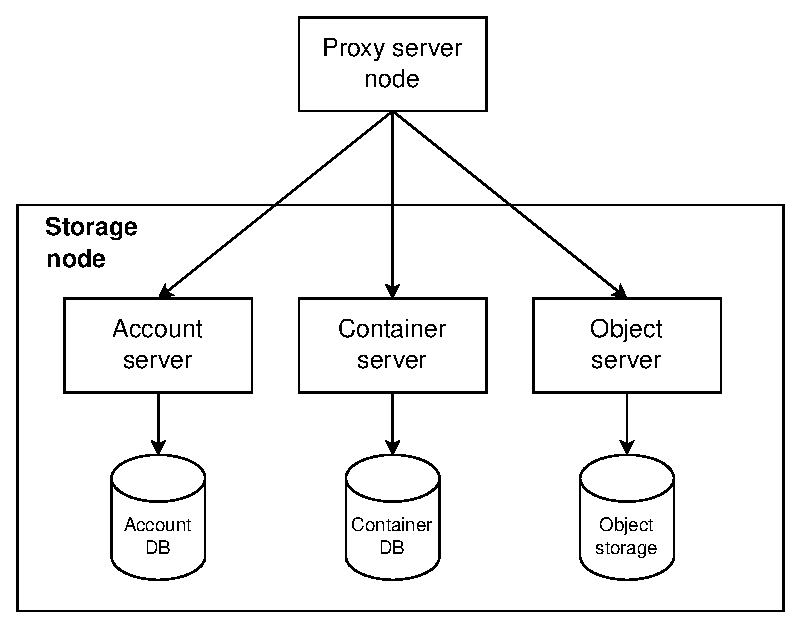
\includegraphics[width=0.90\linewidth]{images/swift-servers.eps}
		\caption{OpenStack Swift servers architecture.}
		\label{fig:swiftServers}
\end{figure}


\subsection{Middleware}
Using Python WSGI middleware, users can add functionalities and behaviors to OpenStack Swift. Most middlewares are added to the Proxy server but can also be part of other servers (account server, container server, or object server).

Middlewares are added by changing the configuration of servers. Listing \ref{lst:swiftMiddleware} is shows how to add \textit{webhook middleware} to proxy server by chaning its pipeline (\textit{pipeline:main}). Middlewares are executed in the given order (first will be called webhook middleware, then proxy-server middleware).

Some of the middlewares are required and will be automatically inserted by swift code\cite{swiftMiddleware}.

\lstset{
		caption=Example of proxy server configuration (proxy-server.conf).,
		label=lst:swiftMiddleware
}
\begin{lstlisting}
[DEFAULT]
log_level = DEBUG
user = <your-user-name>

[pipeline:main]
pipeline = webhook proxy-server

[filter:webhook]
use = egg:swift#webhook

[app:proxy-server]
use = egg:swift#proxy
\end{lstlisting}

\textbf{Interface} - OpenStack Swift servers are implemented using Python WSGI applications. Therefore only Python WSGI middlewares are accepted in OpenStack Swift.

Listing \ref{lst:swift-healthcheck} provides example of simplified \textit{healthcheck middleware}. The constructor takes two arguments, the first is a WSGI application, and the second is a configuration of middleware defined using Python Paste framework in \textit{proxy-server.conf}. Middleware must have a call method containing the request environment information and response from previously called middleware. Middleware can perform some operations and call the next middleware in the pipeline or intercept a request. In the healtcheck example, if the path directs to \texttt{/healtcheck} , the middleware will return \texttt{HTTP Response}, and other middlewares in the pipeline will not be called.

Method \texttt{filter\_factory} is used by the Python Paste framework to instantiate middleware.

\begin{lstlisting}[language=Python, style=pythonStyle, caption=Example of healthcheck middleware in OpenStack Swift, label=lst:swift-healthcheck]
import os
from swift.common.swob import Request, Response

class HealthCheckMiddleware(object):
  def __init__(self, app, conf):
    self.app = app

  def __call__(self, env, start_response):
    req = Request(env)
    if req.path == '/healthcheck':
      return Response(request=req, body=b"OK", content_type="text/plain")(env, start_response)
    return self.app(env, start_response)

def filter_factory(global_conf, **local_conf):
  conf = global_conf.copy()
  conf.update(local_conf)

  def healthcheck_filter(app):
    return HealthCheckMiddleware(app, conf)
  return healthcheck_filter
\end{lstlisting}

\subsection{Metadata}
OpenStack Swift separates metadata into 3 categories based on their use:

\textbf{\texttt{User Metadata}} - User metadata takes form \\
\centerline{\texttt{X-<type>-Meta-<key>:<value>}}\\ where \texttt{<type>} represent resource type(i.e. account, container, object), and \texttt{<key>} and \texttt{<value>} are set by user. User metadata remain persistent until are updated using new value or removed using header \texttt{X-<type>-Meta-<key>} with no value or a header \texttt{X-Remove-<type>-Meta-<key>:<ignored-\\-value>}.

\textbf{\texttt{System Metadata}} - System metadata takes form \texttt{X-<type>-Sysmeta-<key>:<value>}\\ where \texttt{<type>} represent resource type(i.e. account, container, object) and \texttt{<key>} and \texttt{<value>} are set by internal service in Swift WSGI Server.
		All headers containing system metadata are deleted from a client request.

		System metadata are visible only inside Swift, providing a means to store potentially sensitive information regarding Swift resources.

\textbf{\texttt{Object Transient-Sysmeta}} - This type of metadata have form of \texttt{X-Object-Transient-\\-Sysmeta-<key>:<value>}. Transient-sysmeta has a similar behavior as system metadata and can be accessed only within Swift, and headers containing Transient-sysmeta are dropped. If middleware wants to store object metadata, it should use transient-sysmeta\cite{swiftMiddleware}.


\section{Existing solutions}
%\textbf{[Existing solutions]} Discuss existing solutions, be fair in identifying their strengths and weaknesses. Cite important works from the field of your topic. Try to define well what is the \textit{state of the art}. You can include a Section 2 titled ``Background'' or ``Previous Works'' and have the details there and make this paragraph short. Or, you can enlarge this paragraph to a whole page. In many scientific papers, \emph{this} is the most valuable part if it is written properly.
There is no official OpenStack solution that satisfies all requirements mentioned in section \ref{introduction}, although some of existing programs can be used to partially solve some of the problems.

\textbf{Webhook middleware} described in \ref{swiftMiddleware} can be used for detection of new objects in specific container. With some tweaks it could be able to detect object deletion and modifying too. One of many limitations of this middleware is lack of support different destinations (it can pubslish notification only to single type of destination), no filtering, single type of event notification structure and incompatibility with AWS S3.

\textbf{OpenStack Swift attempts} - OpenStack Swift is aware of lack of event notifications and in order to solve it they crated specification for this problem\cite{swiftProblem}. This specification was mainly focused on detection changes inside specific container (creation, modifying and deletiton of objects). There were two attempts to solve this problem.
\begin{itemize}
	\item \textbf{First attempt}\ref{swiftFirstAttempt} - allowed sending notifications only to Zahar[todo] queue and had very simple event notification strucuture. Notification contained only informations about names of account, container and object on which event occured and name of HTTP method.
	\item \textbf{Second attempt}\ref{swiftSecondAttempt} - was more sophisticated solution that was design to support multiple destinations to which notfication can be published. Event notification structure was expanded for informations such as eTag (MD5 checksum) and transaction id. Author introduced concept of "notification policy", which represented configuration of event notifications. One of main critiques made by code reviewers was incompatibility with AWS S3 storage.
\end{itemize}

Both attempts are outdated and due to lack of interest from users/operators OpenStack Swift halted development for this problem.

%\textbf{[Our solution]} Make a quick outline of your approach -- pitch your solution.  The solution will be described later in detail, but give the reader a very quick overview now.

\textbf{ENOSS} - my solution, code name ENOSS, satisfies all requirements specified in section \ref{introduction}. Key features are: events filtering, support of multiple destinations, AWS S3 compatibility, different event notification structure, definition of interfaces for future expansions and different filters, destinations and event notification structure, and design that allows its effortless expansions. %todo - maybe put it proposed solution? Table \cite{tbl:solutionsCmp} compares key features of existing solution and ENOSS.

\section{ENOSS}

%\textbf{[Contributions]} Sell your solution. Pinpoint your achievements. Be fair and objective.

%\phony{Lorem ipsum dolor sit amet, consectetur adipiscing elit. Integer sit amet neque vel mi sodales interdum nec a mi. Aliquam eget turpis venenatis, tincidunt purus eget, euismod neque. Nulla et porta tortor, id lobortis turpis. Sed scelerisque sem eget ante interdum, vel volutpat arcu volutpat. Aliquam cursus, dolor a luctus. }

\section{Conclusions}
\label{sec:Conclusions}

\textbf{[Paper Summary]} What was the paper about, then? What the reader needs to remember about it?
\phony{Lorem ipsum dolor sit amet, consectetur adipiscing elit. Proin vitae aliquet metus. Sed pharetra vehicula sem ut varius. Aliquam molestie nulla et mauris suscipit, ut commodo nunc mollis.}

\textbf{[Highlights of Results]} Exact numbers. Remind the reader that the paper matters.
\phony{Lorem ipsum dolor sit amet, consectetur adipiscing elit. Sed tempus fermentum ipsum at venenatis. Curabitur ultricies, mauris eu ullamcorper mattis, ligula purus dapibus mi, vel dapibus odio nulla et ex. Sed viverra cursus mattis. Suspendisse ornare semper condimentum. Interdum et malesuada fames ac ante ipsum.}

\textbf{[Paper Contributions]} What is the original contribution of this work? Two or three thoughts that one should definitely take home.
\phony{Lorem ipsum dolor sit amet, consectetur adipiscing elit. Praesent posuere mattis ante at imperdiet. Cras id tincidunt purus. Aliquam erat volutpat. Morbi non gravida nisi, non iaculis tortor. Quisque at fringilla neque.}

\textbf{[Future Work]} How can other researchers / developers make use of the results of this work?  Do you have further plans with this work? Or anybody else?
\phony{Lorem ipsum dolor sit amet, consectetur adipiscing elit. Suspendisse sollicitudin posuere massa, non convallis purus ultricies sit amet. Duis at nisl tincidunt, maximus risus a, aliquet massa. Vestibulum libero odio, condimentum ut ex non, eleifend.}

\section*{Acknowledgements}
I would like to thank my supervisor X. Y. for her help.

%--------------------------------------------------------
%--------------------------------------------------------
%--------------------------------------------------------
%	REFERENCE LIST
%--------------------------------------------------------
%--------------------------------------------------------
\phantomsection
\bibliographystyle{unsrt}
\bibliography{bibliography}

%--------------------------------------------------------
%--------------------------------------------------------
%--------------------------------------------------------
\end{document}
